\documentclass{beamer}

\newcommand{\course}{CS 2340 Objects and Design}
\newcommand{\lesson}{Introduction}
\newcommand{\code}{http://www.cc.gatech.edu/~simpkins/teaching/gatech/cs2340/code}

\author[Chris Simpkins]
{Christopher Simpkins \\\texttt{chris.simpkins@gatech.edu}}
\institute[Georgia Tech] % (optional, but mostly needed)

\date[CS 2340]{}

\subject{\lesson}


% If you have a file called "university-logo-filename.xxx", where xxx
% is a graphic format that can be processed by latex or pdflatex,
% resp., then you can add a logo as follows:

% \pgfdeclareimage[width=0.6in]{coc-logo}{cc_2012_logo}
% \logo{\pgfuseimage{coc-logo}}

\mode<presentation>
{
  \usetheme{Berlin}
  \useoutertheme{infolines}

  % or ...

 \setbeamercovered{transparent}
  % or whatever (possibly just delete it)
}

\usepackage{hyperref}
\usepackage{fancybox}
\usepackage{listings}
\usepackage[abbr]{harvard}

\usepackage[english]{babel}
% or whatever

\usepackage[latin1]{inputenc}
% or whatever

\usepackage{times}
\usepackage[T1]{fontenc}
% Or whatever. Note that the encoding and the font should match. If T1
% does not look nice, try deleting the line with the fontenc.


\usepackage{listings}
 
% "define" Scala
\lstdefinelanguage{scala}{
  morekeywords={abstract,case,catch,class,def,%
    do,else,extends,false,final,finally,%
    for,if,implicit,import,match,mixin,%
    new,null,object,override,package,%
    private,protected,requires,return,sealed,%
    super,this,throw,trait,true,try,%
    type,val,var,while,with,yield},
  otherkeywords={=>,<-,<\%,<:,>:,\#,@},
  sensitive=true,
  morecomment=[l]{//},
  morecomment=[n]{/*}{*/},
  morestring=[b]",
  morestring=[b]',
  morestring=[b]""",
}

\usepackage{color}
\definecolor{dkgreen}{rgb}{0,0.6,0}
\definecolor{gray}{rgb}{0.5,0.5,0.5}
\definecolor{mauve}{rgb}{0.58,0,0.82}
 
% Default settings for code listings
\lstset{frame=tb,
  language=scala,
  aboveskip=2mm,
  belowskip=2mm,
  showstringspaces=false,
  columns=flexible,
  basicstyle={\scriptsize\ttfamily},
  numbers=none,
  numberstyle=\tiny\color{gray},
  keywordstyle=\color{blue},
  commentstyle=\color{dkgreen},
  stringstyle=\color{mauve},
  frame=single,
  breaklines=true,
  breakatwhitespace=true,
  keepspaces=true
  %tabsize=3
}


\title[\course] % (optional, use only with long
                                      % paper titles)
{\lesson}

\subtitle{}
%% {Include Only If Paper Has a Subtitle}

\newcommand{\link}[2]{\href{#1}{\textcolor{blue}{\underline{#2}}}}


% \beamerdefaultoverlayspecification{<+->}

\begin{document}

\begin{frame}
  \titlepage
\end{frame}

%------------------------------------------------------------------------
\begin{frame}[fragile]{Course Overview}

\begin{itemize}
\item Workload
\item Course Content
\item Syllabus
\end{itemize}

\end{frame}
%------------------------------------------------------------------------


%------------------------------------------------------------------------
\begin{frame}[fragile]{Expected Time Allotment}

\begin{quote}
One semester credit is expected to require at least three hours of scholarly activity per week.
\end{quote}
 -- \url{http://www.registrar.gatech.edu/faculty/fs_sch.php}\\
\vspace{.1in}
3 credit class = 9 hours a week (~12 in summer)\\
\vspace{.1in}
2.5 hours of lecture (3 x 50min, or 2 x 1:45 = 3.5 hours in summer)\\
\vspace{.1in}
At least 6.5 more hours (8.5 in summer) for reading, studying, and homeworks.

\end{frame}
%------------------------------------------------------------------------

%------------------------------------------------------------------------
\begin{frame}[fragile]{Your Semester Schedule}


\begin{quote}
One semester credit is expected to require at least three hours of scholarly activity per week.
\end{quote}
 -- \url{http://www.registrar.gatech.edu/faculty/fs_sch.php}\\
\vspace{.1in}
12 credit hours = 36 hours a week (49 hours in summer)\\
\vspace{.1in}
Full Time $\ge$ 12 credit hours (including summer)\footnote{\url{http://www.registrar.gatech.edu/students/semestersystem.php}}


\end{frame}
%------------------------------------------------------------------------

\section{Course Content}

%------------------------------------------------------------------------
\begin{frame}[fragile]{CS 2340}

Amalgam of two courses:
\begin{itemize}
\item Software engineering practicum
\begin{itemize}
\item Introduction to software engineering
\item Practical software engineering skills (tools, technologies, practices)
\item Preparation for design capstone (and real jobs)
\end{itemize}
\item Objects and Design
\begin{itemize}
\item Software design principles
\item Object-oriented design
\item Design patterns
\end{itemize}
\end{itemize}

CS 2340 bridges from academia to industry.


\end{frame}
%------------------------------------------------------------------------

\subsection{Tools and Technologies}

%------------------------------------------------------------------------
\begin{frame}[fragile]{"Pro" Java}

\begin{itemize}
\item The classpath
\item Project directory layout
\item Packages
\item Jar files
\item Build automation
\item Using an IDE
\end{itemize}


\end{frame}
%------------------------------------------------------------------------

%------------------------------------------------------------------------
\begin{frame}[fragile]{Web Applications}

\begin{itemize}
\item The HTTP protocol
\item Clients and Servers
\item Java Servlets and JSPs
\item Java web application servers
\end{itemize}

\end{frame}
%------------------------------------------------------------------------

\subsection{Agile Software Development}

%------------------------------------------------------------------------
\begin{frame}[fragile]{Software Engineering}

\begin{itemize}
\item Software development life cycle
\item Waterfall process models
\item Iterative process models
\item Methods for software design, implementation, and testing
\end{itemize}


\end{frame}
%------------------------------------------------------------------------

%------------------------------------------------------------------------
\begin{frame}[fragile]{Agile Development}

Agile Practices
\begin{itemize}
\item Pair programming
\item Clean code
\item Unit testing
\item Simple design
\item Refactoring
\end{itemize}
Agile project management (Scrum)
\begin{itemize}
\item Team roles
\item User stories
\item Small releases
\item Estimation
\end{itemize}


\end{frame}
%------------------------------------------------------------------------

\subsection{Object-oriented Design}

%------------------------------------------------------------------------
\begin{frame}[fragile]{Software Design}

\begin{itemize}
\item Design principles
\item Design techniques
\item System architectures
\item Design documentation
\end{itemize}


\end{frame}
%------------------------------------------------------------------------

%------------------------------------------------------------------------
\begin{frame}[fragile]{Object-Oriented Design}

\begin{itemize}
\item {\bf S}ingle Responsibility Principle
\item {\bf O}pen Closed Principle
\item {\bf L}iskov Substitution Principle
\item {\bf I}nterface Segregation Principle
\item {\bf D}ependency Inversion Principle
\end{itemize}

\end{frame}
%------------------------------------------------------------------------

%------------------------------------------------------------------------
\begin{frame}[fragile]{Design Patterns}

\begin{columns}[c]

\begin{column}{2in}
\begin{center}
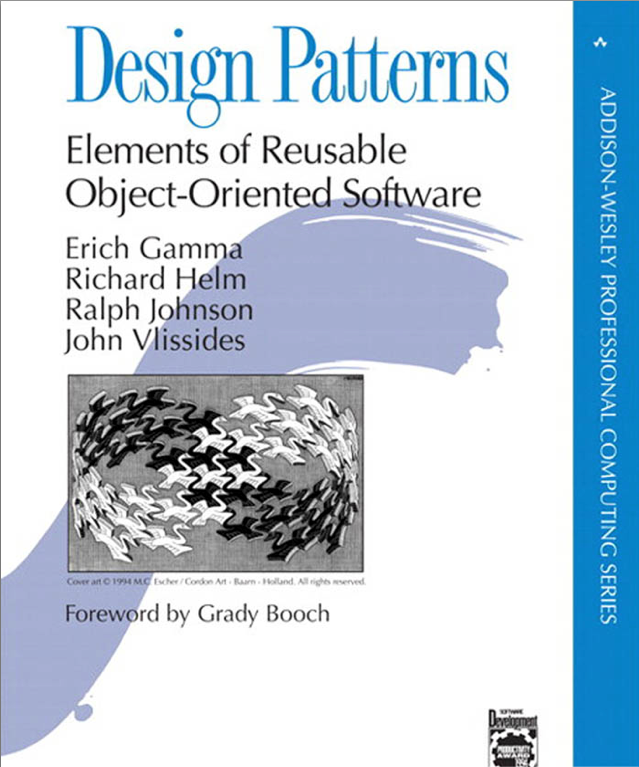
\includegraphics[width=1.9in]{design-patterns-book.png}
\end{center}
\end{column}

\begin{column}{3in}
A recurring object-oriented design.
\begin{itemize}
\item Make proven techniques more accessible to developers of new systems -- don't have to study other systems.
\item Helps in choosing designs that make the system more reusable.
\item Facilitate documenentation and communication with other developers.
\end{itemize}
Design pattern catalog: descriptions of communicating objects and classes that are customized to solve a general design problem in a particular context.

\end{column}

\end{columns}

\end{frame}
%------------------------------------------------------------------------

% %------------------------------------------------------------------------
% \begin{frame}[fragile]{}


% \begin{lstlisting}[language=Python]

% \end{lstlisting}


% \end{frame}
% %------------------------------------------------------------------------

\end{document}
